\documentclass[12pt, a4paper]{article}
\title{Скин-эффект (3.7.1)}
\author{Гаянов Артём, Б02-312}
\date{}
% !TeX encoding = UTF-8

\usepackage{geometry}
\usepackage{amsmath, amsfonts, amssymb, amsthm} % стандартный набор AMS-пакетов для математ. текстов
\usepackage{mathtext}
\usepackage[utf8]{inputenc} % кодировка utf8
\usepackage[russian]{babel} % русский язык
\usepackage[pdftex,dvipsnames]{xcolor} % работа с цветами
\usepackage[pdftex]{graphicx} % графика (картинки)
\usepackage{tikz,pgfplots} % рисунки
\usepackage{indentfirst}
%\usepackage[labelfont=bf,labelsep=endash,skip=3pt]{caption} % подпись картинок
% \usepackage{fancyhdr,pageslts} % настройка колонтитулов
\usepackage{enumitem} % работа со списками
\usepackage{floatrow,multicol,multirow,longtable,hhline} % работа с таблицами
\usepackage{float,wrapfig} % плавающие объекты
\usepackage{tcolorbox} % рамка вокруг текста
%\usepackage[calc]{datetime2} % дата
\usepackage{bm} % жирное начертание в формулах
\usepackage{physics} % физический пакет
\DeclareMathAlphabet\mathbfcal{OMS}{cmsy}{b}{n}
\usepackage{pgfornament} % красивые рюшечки и вензеля
\usepackage{mdframed}
\usepackage{derivative}
\usepackage{mathrsfs} %EDS
\usepackage{soul} % strikethorugh
%\usepackage{boondox-cal}

% ----------------------------------------
% Настройка шрифта

% Просто закооментируйте следующую строчку, если не работает. Будет другой шрифт, правда :(
% \usepackage{pscyr}

% ----------------------------------------
% Стилевые настройки

\usepackage{boldline} % жирная линия после таблиц (чтобы не было ошибок, этот пакет должен подключаться именно тут!)
\floatsetup[table]{style=Plaintop,floatrowsep=qquad} % настройка оформления таблиц
\setlist[enumerate,itemize]{leftmargin=5mm,itemindent=10mm,itemsep=0mm,
listparindent=0em,labelsep=2mm,topsep=2mm,labelwidth=4mm} % настройки списков

\setlength{\columnsep}{0.5cm} % расстояние между колонками
\setlength{\parskip}{1pt} % расстояние до текста от колонтитула

%\usepackage{titlesec} % управление оформлением section
%\renewcommand{\thesection}{\Roman{section}}
%\titleformat{\section}[block]{\bfseries\large}{\thesection.}{5pt}{}

% ----------------------------------------
% Настройки полей
\geometry{
  left=10mm,
  top=10mm,
  right=10mm,
  bottom=15mm,
  marginparsep=0mm,
  marginparwidth=0mm,
  headheight=0pt,
  headsep=0pt,
footskip=20pt}

% ----------------------------------------
% Настройки колонтитулов и нумерации страниц
\pagenumbering{arabic}



\newcounter{ntask}
\setcounter{ntask}{0}


\newcommand{\arsh}{\mathrm{arsh} \,\,}
\newcommand{\arch}{\mathrm{arch} \,\,}
\newcommand{\arth}{\mathrm{arth} \,\,}
\newcommand{\arcth}{\mathrm{arcth} \,\,}
\renewcommand{\Re}{\operatorname{Re} \,}
\newcommand{\EDS}{\mathscr{E}}
\newcommand{\diffract}[1]{\frac{\mathrm{d}#1}{\mathrm{d}t}}



\newcommand{\V}{~\mathrm{V}}
\newcommand{\mV}{~\mathrm{mV}}
\newcommand{\A}{~\mathrm{A}}
\newcommand{\mA}{~\mathrm{mA}}
\newcommand{\uT}{~\mathrm{\mu T}}
\newcommand{\mT}{~\mathrm{mT}}
\newcommand{\kHz}{~\mathrm{kHz}}
\newcommand{\Hz}{~\mathrm{Hz}}
\newcommand{\mm}{~\mathrm{mm}}

\addto\captionsrussian{\def\refname{Источники}}

\begin{document}
\maketitle

\section{Цель работы}
Исследовать явление проникновение переменного магнитного поля в медный полый цилиндр. 

\section{Теоретические сведения}
\subsection*{Скин-эффект для полупрастранства}
\vspace{1cm}
\begin{wrapfigure}{l}{0.3\textwidth}
  \begin{center}
    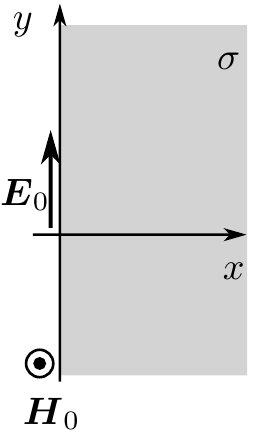
\includegraphics[width=0.8\textwidth]{pics/poluprostranstvo}
  \end{center}
  %\caption{Скин-эффект в полупространстве}\label{fig:poluprostranstvo}
\end{wrapfigure}

Рассмотрим квазистационарное поле внутри проводящей среды в простейшем плоском случае.
Пусть вектор $\vb*{E}$ направлен всюду вдоль оси $y$ и зависит только от координаты $x$, т. е. ${E_x} = {E_z} \equiv 0$, $E_y=E_y(x,t)$.
В квазистационарном приближении
\begin{equation*}
  \grad \times \vb*{H} = \sigma \vb*{E}
\end{equation*}

Преобразуя это уравнение, можно получить уравнение, схожее с уравнением диффузии:
\begin{equation}
  \grad^2\vb*{H}=\sigma\mu\mu_0 \frac{\partial \vb*{H}}{\partial t}\label{eq:laplacian_H}
\end{equation}
Точно такое же уравнение имеет место и для вектора $E:$
\begin{equation}
  \grad^2\vb*{E}=\sigma\mu\mu_0 \frac{\partial \vb*{E}}{\partial t}\label{eq:diffusion}
\end{equation}

Подставляем в (\ref{eq:diffusion}) наше электрическое поле $E_y=E_y(x,t)$
\begin{equation}
  \frac{\partial^2 E_y}{\partial x^2} = \sigma\mu\mu_0\frac{\partial E_y}{\partial t}
  \label{eq:diffusion_chastni}
\end{equation}
Если $E_y(0,t)=E_0 e^{i\omega t}$ то решением (\ref{eq:diffusion_chastni}) будет функция вида
\begin{equation}
  E_y(x,t)=E_0 e^{-x/\delta} e^{i(\omega t - x/\delta)}
  \label{eq:skin_effect_poluprostranstvo}
\end{equation}
где
\begin{equation}
  \delta = \sqrt{\frac{2}{\omega\sigma\mu\mu_0}}
  \label{eq:delta}
\end{equation}

\newpage
\subsection*{Скин-эффект в тонком полом цилиндре}
\vspace{0cm}
\begin{wrapfigure}[30]{l}{0.3\textwidth}
  \vspace{-7mm}
  \begin{center}
    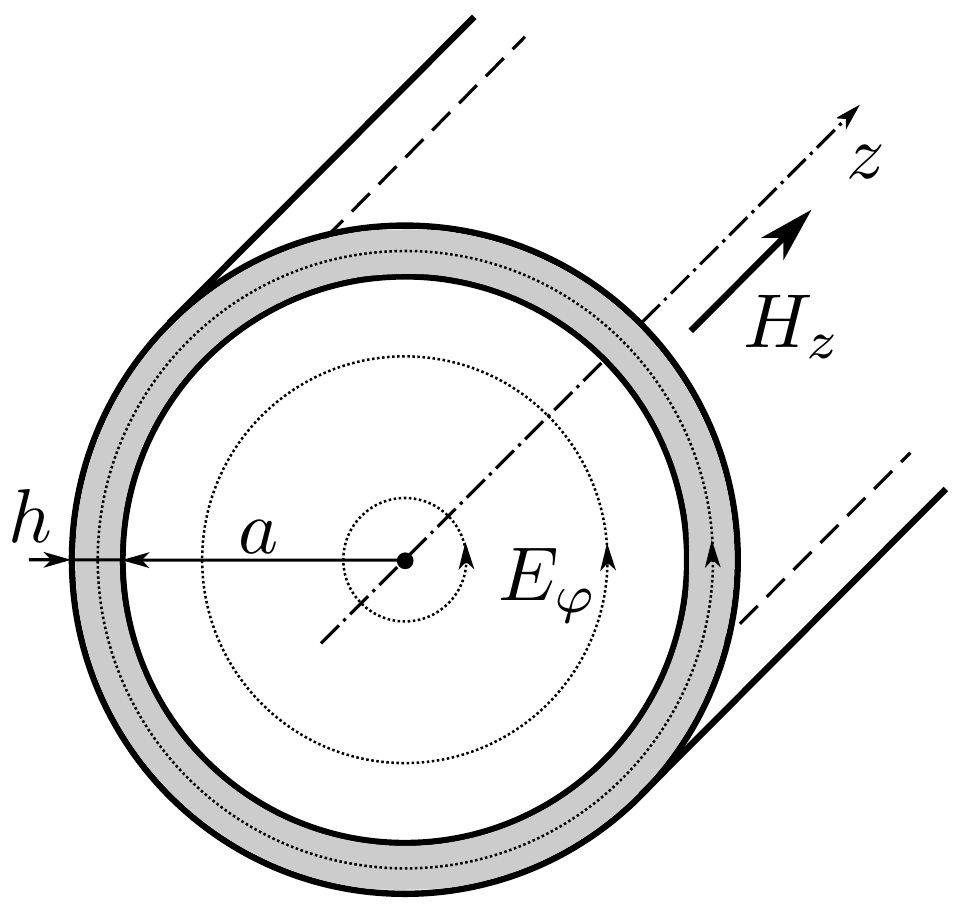
\includegraphics[width=0.8\textwidth]{pics/cilindr}
  \end{center}
  \caption{Эл-магнитные поля в цилиндре и у стенки}\label{fig:cilindr}

  \begin{center}
    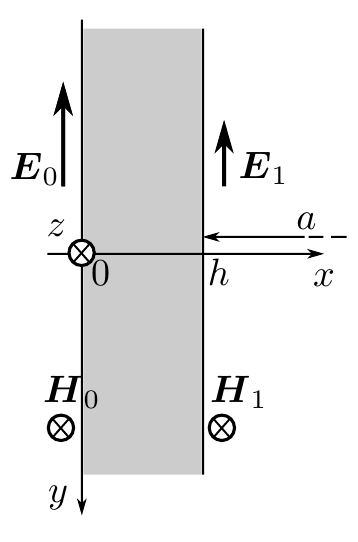
\includegraphics[width=0.8\textwidth]{pics/stenka}
  \end{center}
  \label{fig:stenka}
\end{wrapfigure}

Перейдем теперь к описанию теории в нашей работе. Из соображении симметрии и
непрерывности соответствующих компонет векторов $\vb*{E}$ и $\vb*{H}$ можем сказать что
\begin{equation*}
  H_z = H(r)e^{i\omega t} \text{, } E_\varphi = E(r)e^{i\omega t}
\end{equation*}
и при этом функции $H(r)$ и $E(r)$ непрерывны.

Внутри цилиндра токов нет, следовательно $H(r)=H_1=\text{const}$ внутри цилиндра.
По теореме об электромагнитной индукции
\begin{equation*}
  E(r) = -\frac{1}{2}\mu_0 r \cdot i \omega H_1
\end{equation*}
откуда мы получаем граничное условие
\begin{equation}
  E_1=E(a)= -\frac{1}{2}\mu_0 a \cdot i \omega H_1
  \label{eq:granichnoe_uslovie_E}
\end{equation}

В прближении $h \ll a$ можем пренебречь кривизной стенки и смоделировать
его бесконечной полосой. Тогда, надо решить уравнение (\ref{eq:laplacian_H})
с граничными условиями. Решая уравнение получим связь полей $H_1$
(поле внутри цилиндра которое мы будем измерять) и $H_0$, которое колебается с частотой
$\omega$

\begin{equation}
  H_1 = \frac{H_0}{\ch(\alpha h) + \frac{1}{2} \alpha a \sh(\alpha h)}
  \text{\ \ \ }
  \alpha = \sqrt{i\omega \sigma \mu_0} = \frac{\sqrt{2}}{\delta}e^{i\pi/4}
  \label{eq:svyaz_poley}
\end{equation}

из этой формулы получим сколько по фазе отстает поле $H_1$ от $H_0$. При $\delta \ll h$
(высокачастотная область)

\begin{equation}
  \psi \approx \frac{\pi}{4} + \frac{h}{\delta} =
  \frac{\pi}{4} + h \sqrt{\frac{\omega \sigma \mu_0}{2}}
  \label{eq:faza_high_freq}
\end{equation}

При $\delta \gg h$ (низкочастотная область)

\begin{equation}
  \tan \psi \approx \frac{ah}{\delta^2} = \pi a h \sigma \mu \mu_0 f
  \label{eq:phase_low_freq}
\end{equation}
и кроме того
\begin{equation}
  \left(\frac{|H_1|}{|H_0|}\right)^2 = \dfrac{1}{1 + \frac{1}{4}(ah\sigma \mu_0 \omega)^2}
  \label{eq:low_freq_ampl}
\end{equation}

\subsection*{Влияние скин-эффекта на индуктивность катушки}
Из-за скин эффекта индуктивность соленоида с медным цилиндрическим экраном
внутри будет зависеть от частоты тока. На высоких частотах магнитное поле не проника
ет внутрь соленоида (за экран), поэтому суммарный магнитный поток, пронизывающий
катушку, уменьшается, и, соответственно, уменьшается и индуктивность катушки. Можно показать,
что индуктивность катушки зависит от частоты как:
\begin{equation}
  \frac{L_\text{max} - L}{L - L_\text{min}} = (\pi ah \mu_0 \sigma f)^2
  \label{eq:ind_of_freq}
\end{equation}
\section{Методика измерений}
\textbf{В работе используются:} генератор сигналов АКИП–3420, соленоид,
намотанный на полый цилиндрический каркас, медный экран в виде полого цилиндра,
измерительная катушка, ам­перметр, вольтметр, двухканальный осциллограф GOS–620, RLC-метр.

\begin{wrapfigure}[13]{l}{0.4\textwidth}
  \centering
  \vspace{-8mm}
  \begin{center}
    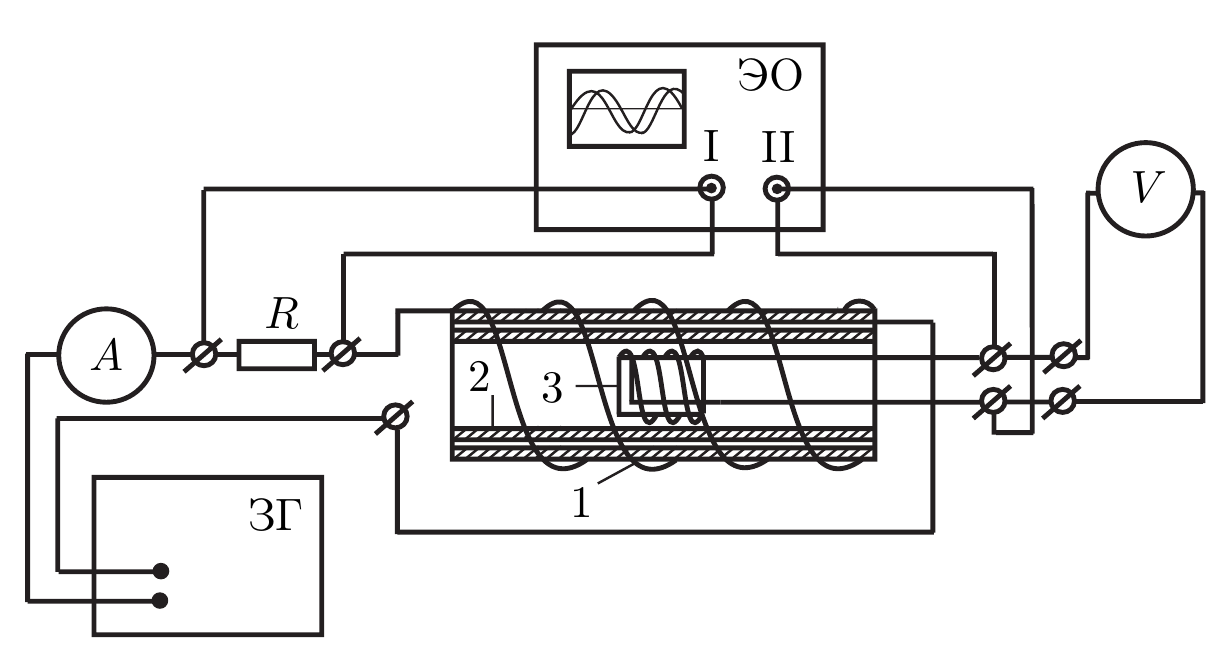
\includegraphics[width=0.8\textwidth]{pics/setup}
  \end{center}
  \caption{Установка}\label{fig:ustanovka}
\end{wrapfigure}

Переменное магнитное поле создается соленоидом 1, на который подается переменный ток со звукового генератора ЗГ. Внутри соленоида расположен медный экран 2. Магнитное поле внутри цилиндра измеряется катушкой 3. Напряжение на катушке пропорциональна производной $\dot{B_1}(t)$
\begin{equation*}
  U(t) \propto \dot{B_1}(t) = -i\omega \mu \mu_0 H_1 e^{i\omega t}
\end{equation*}
Поле внутри цилиндра пропорциональна току через соленоид
\begin{equation*}
  H_0(t) \propto I(t)
\end{equation*}
Отсюда несложно увидеть, что
\begin{equation}
  \frac{\abs{H_1}}{\abs{H_0}} = c \cdot \frac{U}{f I} = \xi / \xi_0
  \label{eq:ampl_share}
\end{equation}
где константу  $\xi_0$ можно определить из условия $\abs{H_1}/\abs{H_0} \rightarrow 1$ при
$\nu \rightarrow 0$.\\

При измерениях разности фаз нужно учесть, что первый сигнал на осциллографе
пропорционален магнитному полю снаружи, а второй пропорционален производному
поля внутри цилиндра по времени, поэтому измеренная на осциллографе разность фаз $\varphi$ будет на $\frac{\pi}{2}$ больше реальной $\psi$:
\[\varphi = \psi + \frac{\pi}{2}\]



\section{Результаты измерений}
\subsection{Измерение амплитуд на малых частотах}
Пользуясь соотношением (\ref{eq:ampl_share}), мы можем снять зависимость $\xi = \frac{U}{fI}$ от $f$
и аппроксимировать её. Результаты приведены в \textit{табл. \ref{Table:low_freq}} и на \textit{рис. \ref{fig:low_freq}}.
\begin{table}[H]
  \begin{tabular}{|l|c|c|c|c|c|}
    \hline
    $f/f_0$ & $f, \kHz$ & $U, \V$ & $I, \mA$ & $\xi$ & $1/\xi^2$ \\
    \hline
    0.012 & 27 & 0.1410 & 379 & 0.01378 & 5267 \\
    0.016 & 36 & 0.1850 & 376 & 0.01367 & 5353 \\
    0.020 & 45 & 0.2260 & 373 & 0.01346 & 5516 \\
    0.024 & 54 & 0.2638 & 369 & 0.01324 & 5705 \\
    0.028 & 63 & 0.2988 & 364 & 0.01303 & 5890 \\
    0.032 & 72 & 0.3307 & 359 & 0.01279 & 6109 \\
    0.036 & 81 & 0.3594 & 354 & 0.01253 & 6365 \\
    0.040 & 90 & 0.3851 & 349 & 0.01226 & 6653 \\
    0.044 & 99 & 0.4082 & 344 & 0.01199 & 6961 \\
    0.048 & 108 & 0.4265 & 338 & 0.01168 & 7326 \\
    \hline
  \end{tabular}
  \caption{Результаты измерения в низкочастотной области}
  \label{Table:low_freq}
\end{table}

\begin{figure}[H]
  \centering
  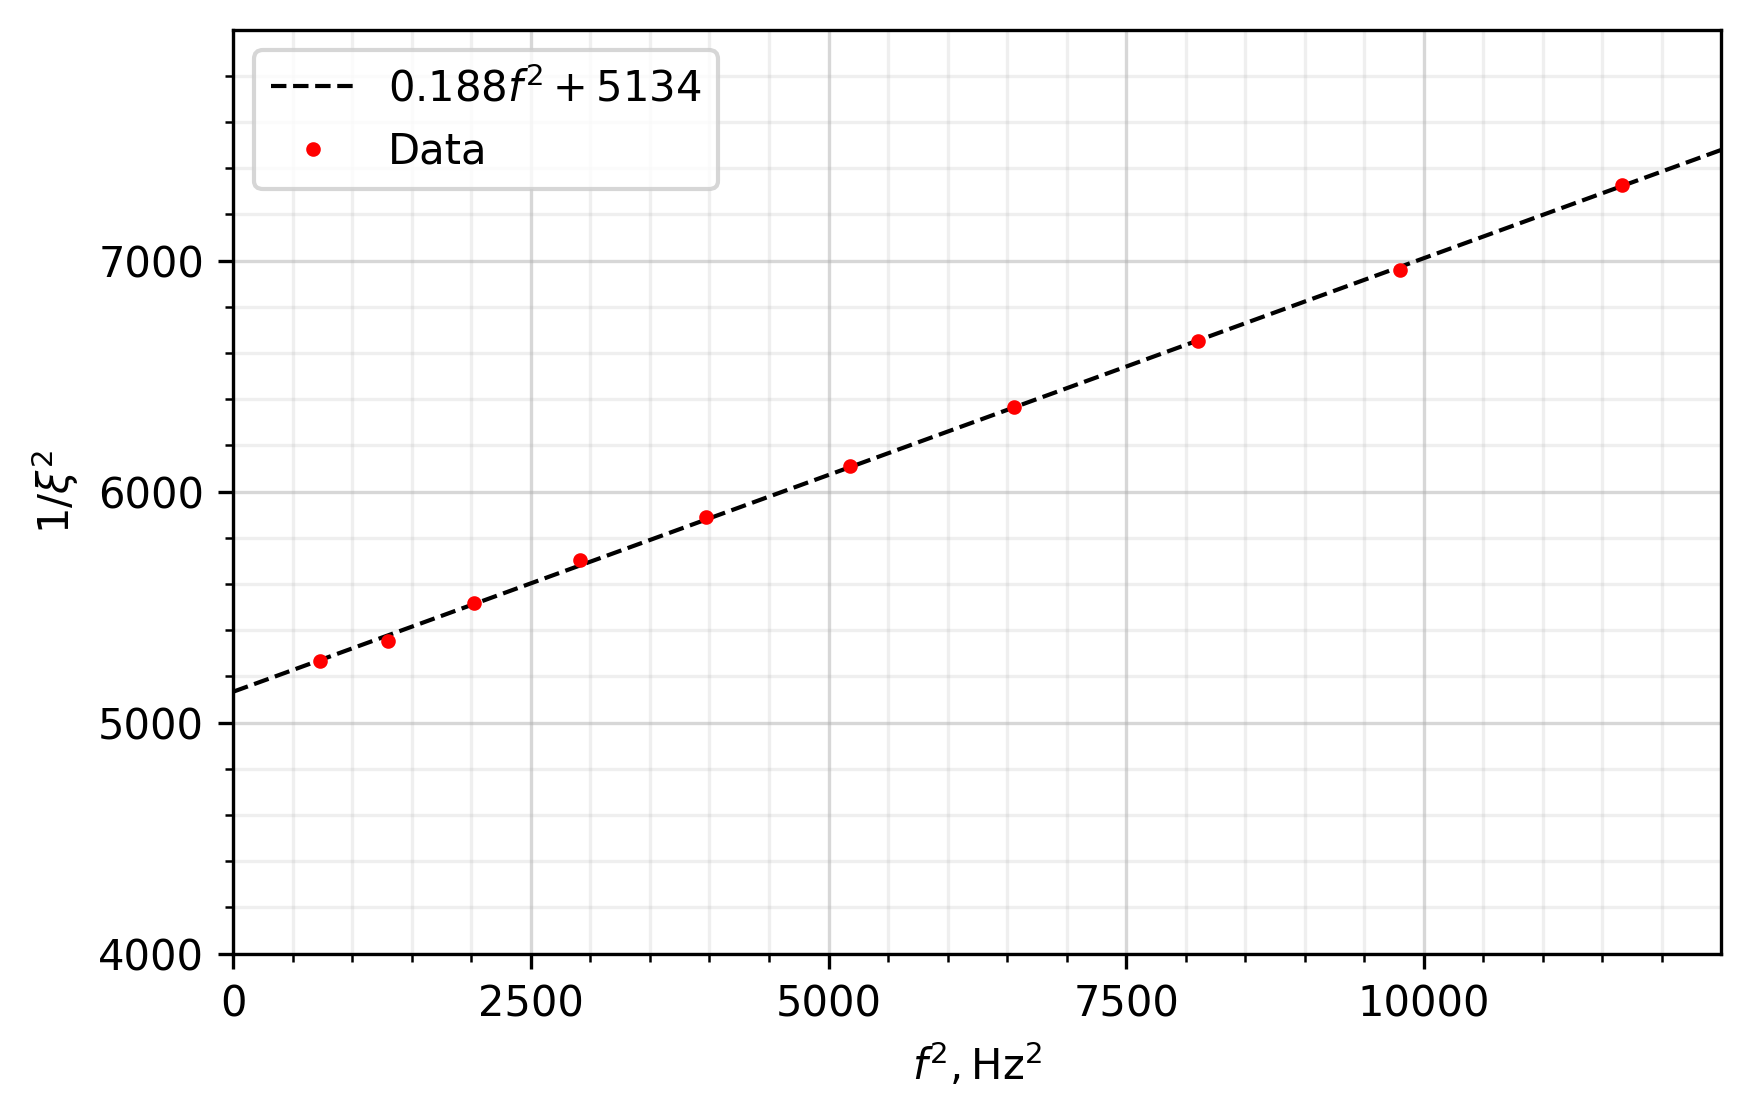
\includegraphics[width=0.6\linewidth]{pics/res7.png}
  \caption{Линеаризация $1/\xi^2 (f^2)$ в пределе малых частот}
  \label{fig:low_freq}
\end{figure}

Тогда просто по своему определению $\xi_0 = \sqrt{\dfrac{1}{5134}} \approx 0.0140$.
Используя (\ref{eq:low_freq_ampl}), найдем проводимость меди из углового коэффициента графика:
\[\tilde{k} = k \cdot \xi_0^2 = 0.188/5134 \Hz^{-2}= 36.6\cdot10^{-6} \Hz^{-2}\]
\[\tilde{k} = (ah\sigma \mu_0 \pi)^2\]
Учтём параметры установки $2a = 45 \mm$, $h = 1.5 \mm$, и рассчитаем $\sigma$:
\[\sigma = 45.4~\mathrm{MSm/m}\]
что хорошо совпадает с оценочным значением в $5\cdot 10^7~\mathrm{Sm/m}$, которое было взято для вычисления $f_0$.
\subsection{Сдвиг фаз на низких частотах}
Аналогично с предыдущим пунктом, согласно (\ref{eq:phase_low_freq}) найдем проводимость меди.
Таблица с данными находится в \textbf{приложении}. Полученный график приведен на \textit{рис. \ref{fig:plot_low_freq}}.
\begin{figure}[H]
  \centering
  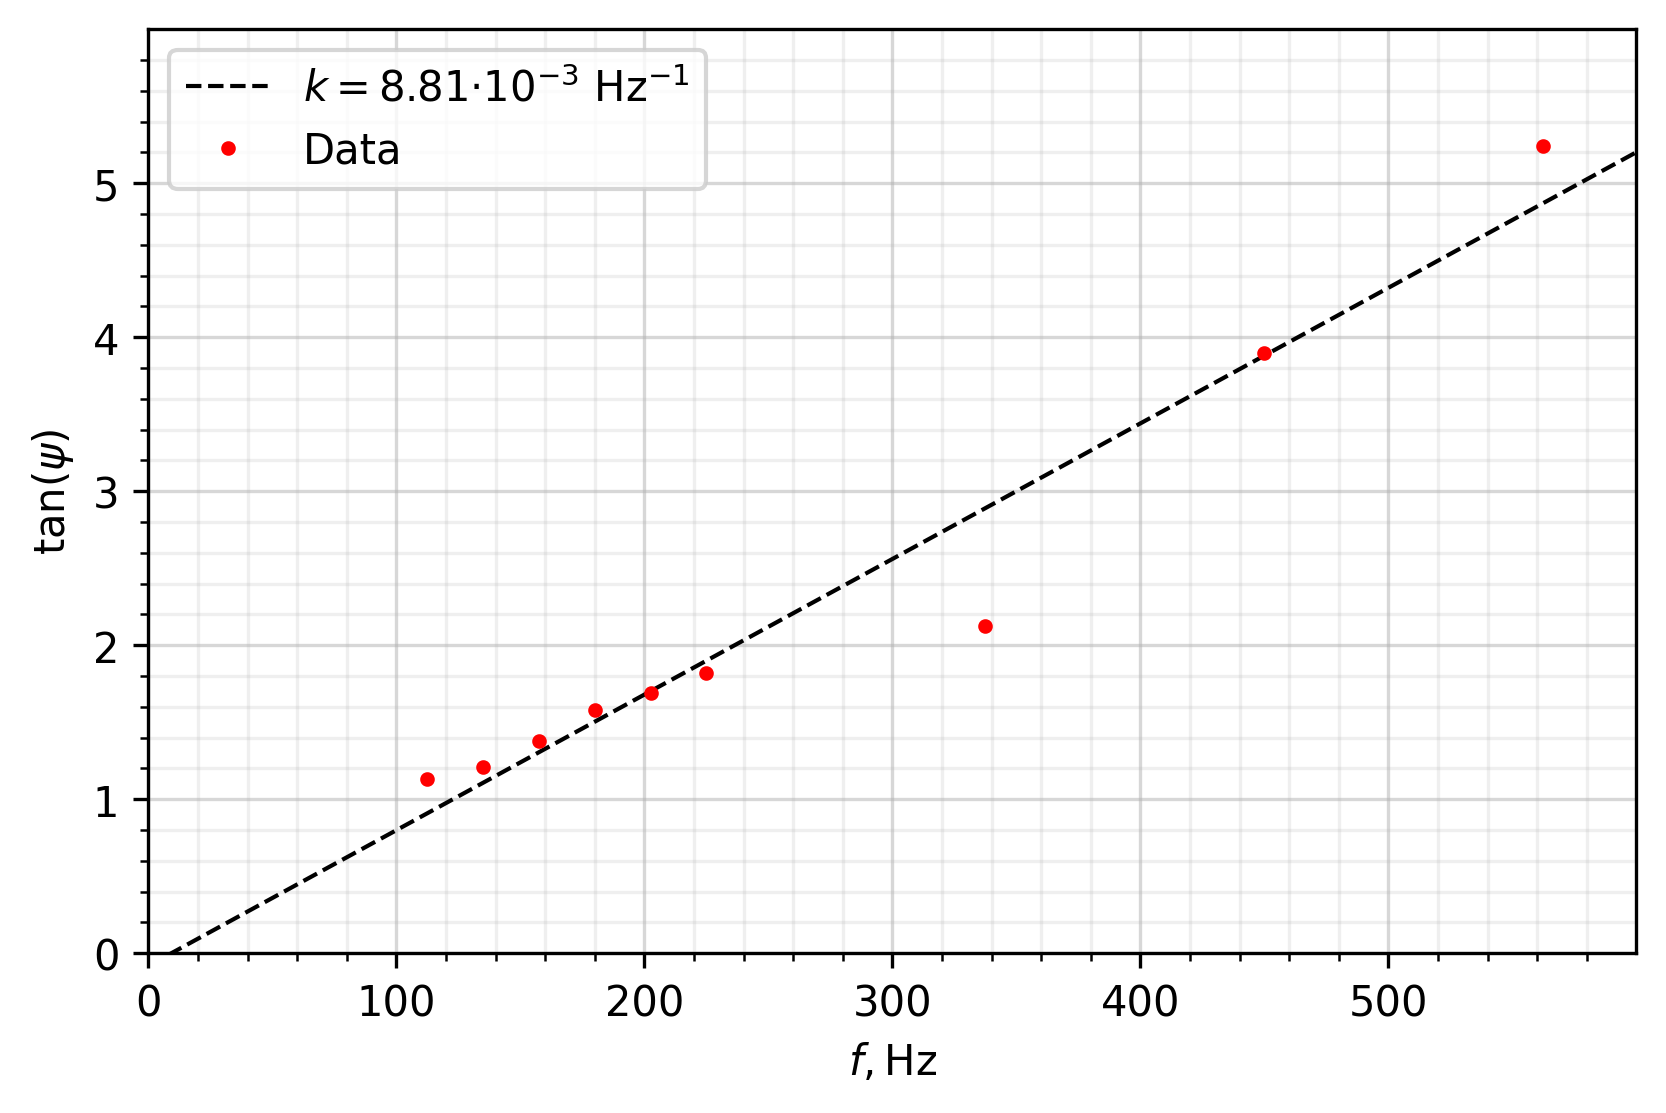
\includegraphics[width=0.6\linewidth]{pics/res8.png}
  \caption{График зависимости фазового сдвига на малых частотах}
  \label{fig:plot_low_freq}
\end{figure}
В целом видно, что зависимость плохо ложится на прямую, но оценки ради можно посчитать соответствующую проводимость меди:
\[\sigma = \dfrac{k}{ah\mu_0 \pi} \approx 66.3 \mathrm{MSm/m}\]

\subsection{Сдвиг фаз на высоких частотах}

Аналогично с предыдущим пунктом, согласно (\ref{eq:faza_high_freq}) найдем проводимость меди.
Таблица с данными находится в \textbf{приложении}. Полученный график приведен на \textit{рис. \ref{fig:plot_high_freq}}.
\begin{figure}[H]
  \centering
  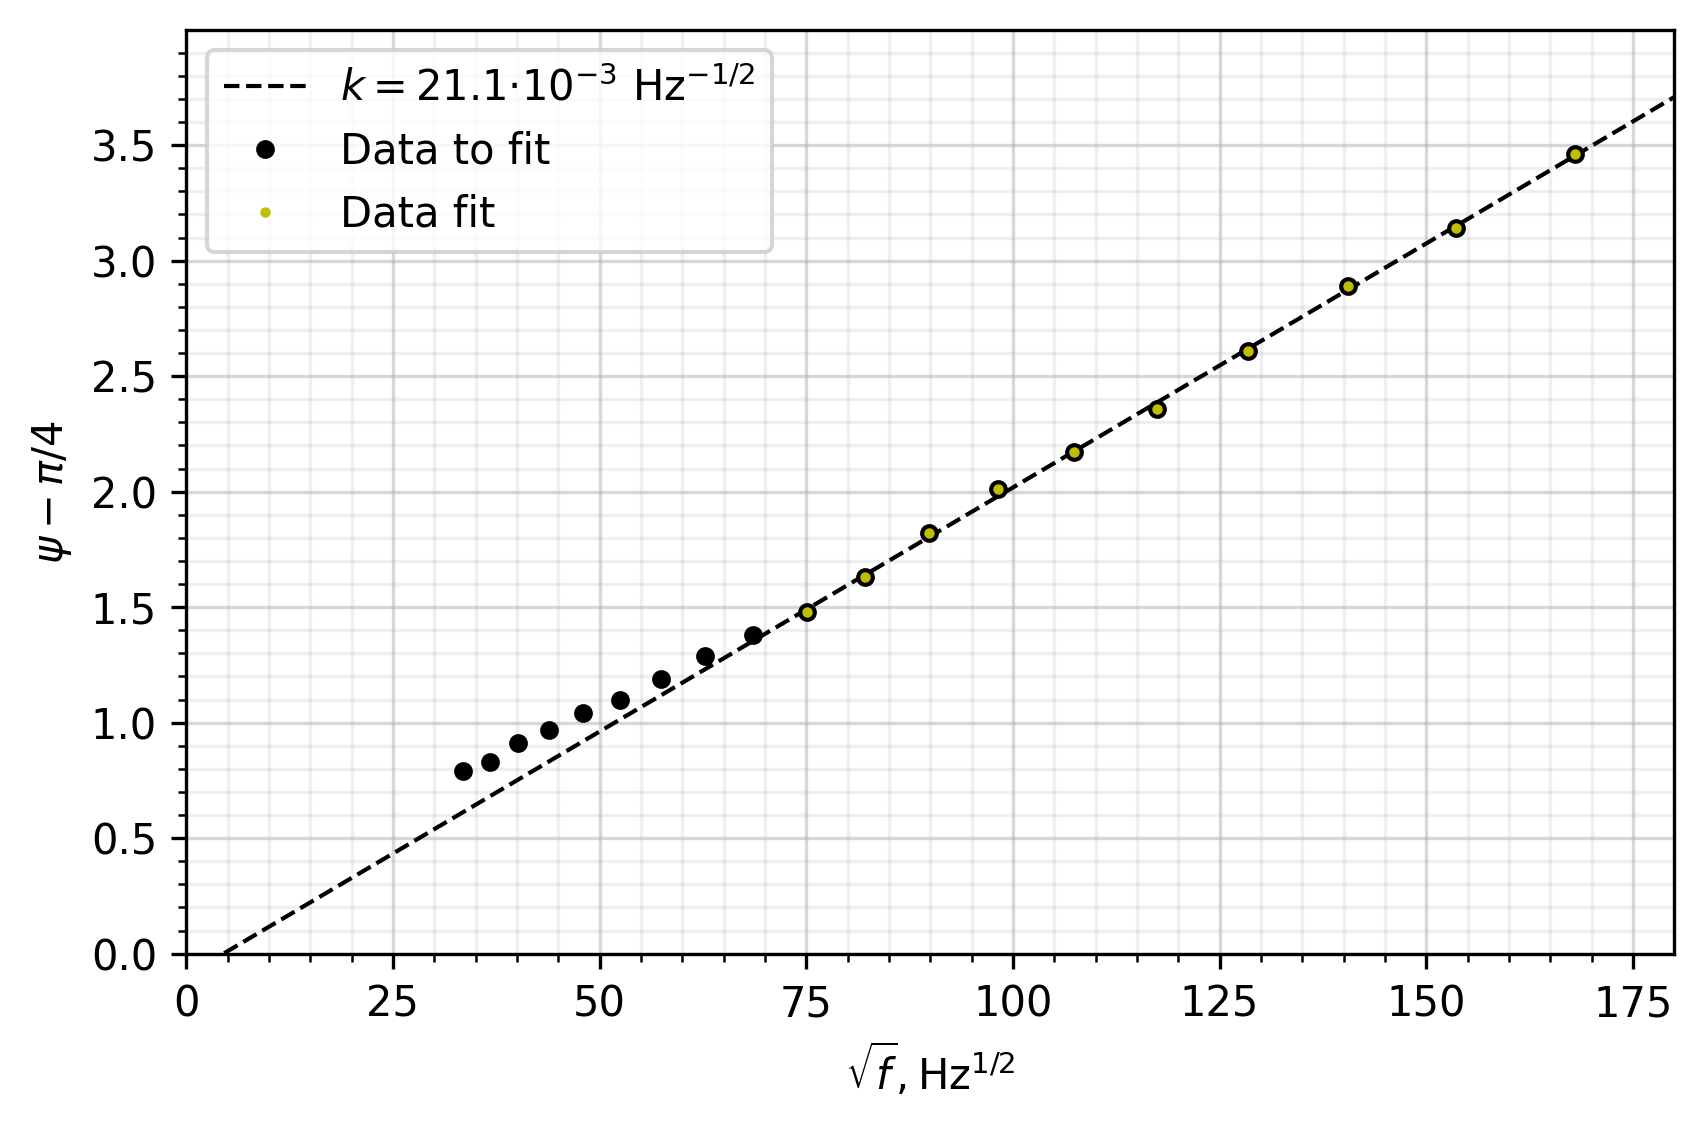
\includegraphics[width=0.6\linewidth]{pics/res9.png}
  \caption{График зависимости фазового сдвига на малых частотах}
  \label{fig:plot_high_freq}
\end{figure}
\[k = h\sqrt{\pi \sigma \mu_0}\]
\[\sigma = \left( \frac{k}{h} \right)^2 \frac{1}{\pi \mu_0} \approx 50.1~\mathrm{MSm/m}\]

\subsection{Изменение индуктивности катушки}
В данном пункте измеряется напрямую RLC-метров зависимость индуктивности катушки от частоты.
Результаты в таблице приводятся в приложении.
\begin{figure}[H]
  \centering
  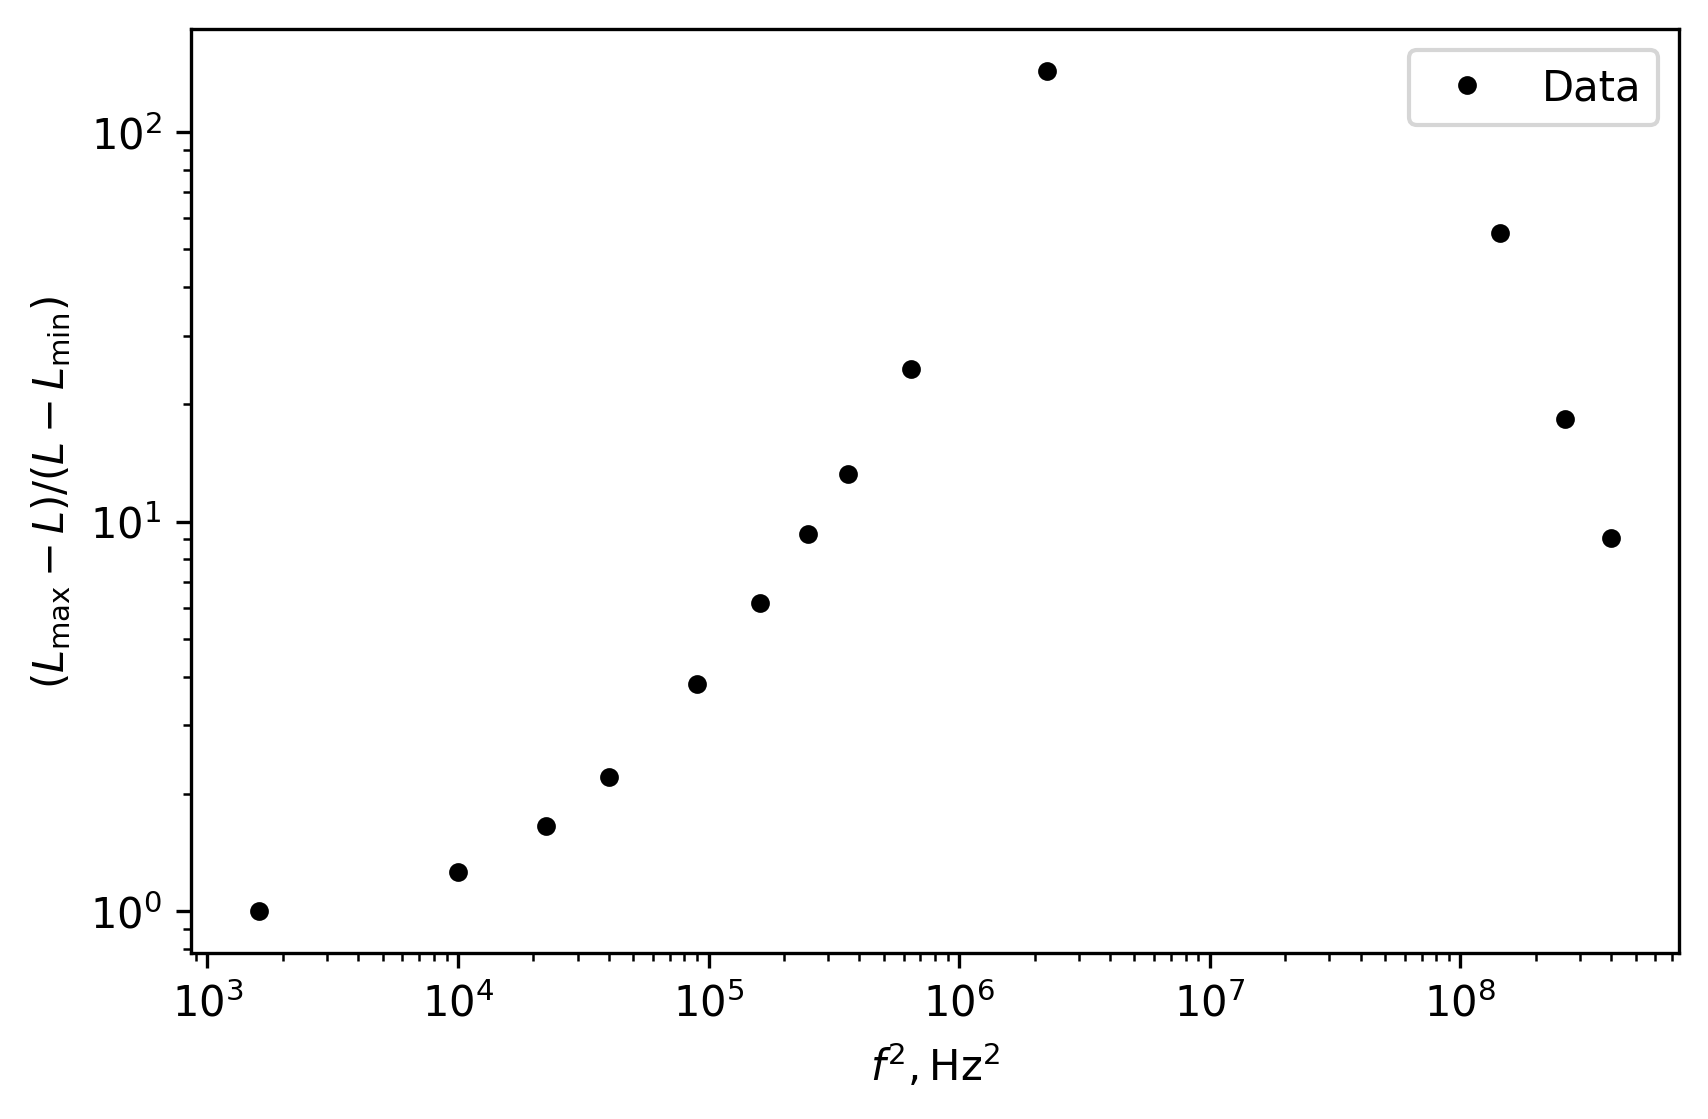
\includegraphics[width=0.6\linewidth]{pics/psi(sqrtf).png}
  \caption{Линеаризованный график зависимости индуктивности катушки от частоты}
  \label{fig:plot_high_freq}
\end{figure}

К сожалению, несмотря на построение в логарифмическом масштабе, обнаружить ожидаемую зависимость не удалось.
\section{Обсуждение результатов и вывод}
В работе был исследован скин-эффект в тонкостенном проводящем цилиндре в приближении малых и больших частот. С помощью косвенных измерений тремя методами найдена проводимость материала цилиндра, которая по порядку совпадает с табличной, максимальное отклонение составило порядка $\sim 30\%$.
Также была выполнена попытка измерения зависимости индуктивности катушки от частоты, но ожидаемого в теории результата пронаблюдать не удалось. Возможно, это связано с собственной ёмкостью катушки, которая влияет на импеданс помимо скин-эффекта.


\section{Приложение}
\begin{table}[h]
  \centering
  \begin{tabular}{|l|c|c|c|c|c|}
    \hline
    $f, \Hz $& $\text{div}(T)$ & $\text{div}(\Delta T)$ & $\psi$ & $\tan{\psi}$ \\
    \hline
    112.5 & 10 & 2.3 & 0.848 & 1.134 \\
    135.0 & 10 & 2.2 & 0.880 & 1.209 \\
    157.5 & 10 & 2.0 & 0.942 & 1.376 \\
    180.0 & 10 & 1.8 & 1.005 & 1.576 \\
    202.5 & 10 & 1.7 & 1.037 & 1.691 \\
    225.0 & 10 & 1.6 & 1.068 & 1.819 \\
    337.5 & 10 & 1.4 & 1.131 & 2.125 \\
    450.0 & 10 & 0.8 & 1.319 & 3.895 \\
    562.5 & 10 & 0.6 & 1.382 & 5.242 \\
    \hline
  \end{tabular}
  \caption{Данные, полученные для фазового сдвига при низких частотах}
  \label{table:phase_low_freq}

\end{table}

\begin{table}[H]
  \begin{tabular}{|l|c|c|c|c|}
    \hline
    $f, \kHz$ & $\psi$ & $\sqrt f, \mathrm{Hz}^{1/2}$ & $\psi - \pi/4$  \\
    \hline
    1.13 & 1.57 & 33.5 & 0.79   \\
    1.35 & 1.61 & 36.7 & 0.83  \\
    1.61 & 1.7 & 40.1 & 0.91  \\
    1.92 & 1.76 & 43.9 & 0.97  \\
    2.3 & 1.82 & 48.0 & 1.04  \\
    2.75 & 1.88 & 52.5 & 1.1  \\
    3.29 & 1.98 & 57.4 & 1.19  \\
    3.94 & 2.07 & 62.8 & 1.29  \\
    4.71 & 2.17 & 68.6 & 1.38  \\
    5.63 & 2.26 & 75.1 & 1.48  \\
    6.74 & 2.42 & 82.1 & 1.63  \\
    8.06 & 2.61 & 89.8 & 1.82  \\
    9.64 & 2.8 & 98.2 & 2.01  \\
    11.53 & 2.95 & 107.4 & 2.17  \\
    13.79 & 3.14 & 117.4 & 2.36  \\
    16.49 & 3.39 & 128.4 & 2.61  \\
    19.73 & 3.68 & 140.5 & 2.89  \\
    23.59 & 3.93 & 153.6 & 3.14  \\
    28.22 & 4.24 & 168.0 & 3.46  \\
    \hline
  \end{tabular}
  \caption{Данные, полученные для фазового сдвига при высоких частотах}
\end{table}

\begin{table}[H]
  \begin{tabular}{|l|r|r|r|}
    \hline
    № & $f, \kHz$ & $L, \mathrm{mH}$ & $\Delta L_{max}/\Delta L_{min}$ \\
    \hline
    0 & 40 & 10.08 & 1.00 \\
    1 & 100 & 8.59 & 1.26 \\
    2 & 150 & 7.24 & 1.66 \\
    3 & 200 & 6.16 & 2.21 \\
    4 & 300 & 4.79 & 3.83 \\
    5 & 400 & 4.08& 6.17 \\
    6 & 500 & 3.69 & 9.30 \\
    7 & 600 & 3.46 & 13.26 \\
    8 & 800 & 3.21 & 24.69 \\
    9 & 1500 & 2.97 & 143.20 \\
    10 & 7500 & 2.92 & --- \\
    11 & 12000 & 3.05 & 55.08 \\
    12 & 16200 & 3.31 & 18.45 \\
    13 & 20000 & 3.71 & 9.06 \\
    \hline
    \end{tabular}
\end{table}

\end{document}
